\subsection{Polyhedra en het bestaande ontwerp}
\noindent {\em Auteur: Bram Vandendriessche}
\\\\
\noindent Het ontwerp van de simulator dat vorig semester tot stand kwam, zorgde ervoor dat de uitbreiding ervan met polyhedra vrij eenvoudig in te voeren was. Door een nieuw type \textit{Polyhedron} dat erft van \textit{WorldObjects}, moesten er in \textit{World} zelf slechts enkele extra methodes ge\"implementeerd worden m.b.t. het toevoegen en verwijderen van een \textit{Polyhedron} aan de bestaande wereld.\\
\\
\noindent 
Een \textit{Polyhedron} zelf is zo ontworpen dat die bestaat uit verschillende \textit{Triangles}. De \texttt{draw()}-methode van de \textit{Polyhedron} draagt elke \textit{Triangle} die tot de Polyhedron behoort, op om zichzelf te tekenen. Een \textit{Triangle} bestaat uit co\"ordinaten voor zijn drie hoekpunten en een kleur voor het buitenste gedeelte van de driehoek. Op basis daarvan worden de binnenste hoekpunten berekend en wordt er een kleur afgeleid uit de kleur van de buitenste driehoek zodat de driehoek voldoet aan de gegeven beperkingen m.b.t. de kleur, zie Tabel \ref{table: HSVwaarden}, en de oppervlakte.\\
\\
\noindent
Het ontwerp van het Testbed heeft de grote zwakte dat het erg moeilijk is om individuele elementen en methodes zoals bijvoorbeeld \textit{Collision Detection}, te testen. Dit komt doordat de objecten erg afhankelijk zijn van de wereld waarin ze bestaan. Die wereld is bovendien altijd afhankelijk van de \textit{gl}-component van \textit{OpenGL}, waardoor het noodzakelijk is een volledige \textit{GL}-wereld op te zetten voor de test kan worden uitgevoerd. Een oplossing hiervoor zou zijn om de objecten en wereld zo op te splitsen dat presentatie en representatie gesplitst worden, zodat het representatie-gedeelte onafhankelijk kan gebruikt worden. Daarnaast zou dan enkel de wereld weet moeten hebben van haar objecten en niet andersom, zodat objecten onafhankelijk van de wereld kunnen worden getest. Deze inzichten werden dan ook toegepast bij het ontwerp van de 3D-component van de Autopilot (zie \ref{sec: 3dAutopilotScan}).\\
\\
\noindent
Voor het testen van de Autopilot zijn verschillende figuren ontworpen. Zij vallen onder \textit{PredefinedPolyhedron}, een subklasse van \textit{Polyhedron} die ook een positie mee kan krijgen bij creatie. Hierdoor kan de figuur naar een gewenste positie worden geplaatst. De gewone Polyhedron (dus de niet vooraf gedefinieerde) krijgen geen 3D-co\"ordinaat mee. Hun positie wordt gezet op het massapunt van de polyhedron, i.e. de gemiddelde 3D-co\"ordinaat van alle hoekpunten. Op die manier wordt gezorgd dat de positie logisch is t.o.v. de hoekpunten. Het is dus niet mogelijk dat de driehoeken van een figuur bijvoorbeeld rond (20,0,0) gedefinieerd worden, maar de polyehdron zelf een positie van (0,0,-40) krijgt toegewezen. De figuren vari\"eren van een eenvoudige piramide met vier hoekpunten tot meer complexe figuren zoals een kubus met een opening in, waarbij de Autopilot zal moeten weten dat het voor de drone niet mogelijk is hierdoor te vliegen, zie Figuur \ref{fig: polyhedra}.

\begin{figure}[H]
	\centering
	\begin{subfigure}{.5\textwidth}
		\centering
		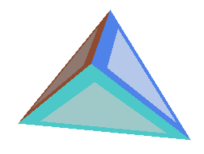
\includegraphics[width=.4\linewidth]{Testbed/4point.png}
		\caption{Eenvoudige figuur}
	\end{subfigure}%
	\begin{subfigure}{.5\textwidth}
		\centering
		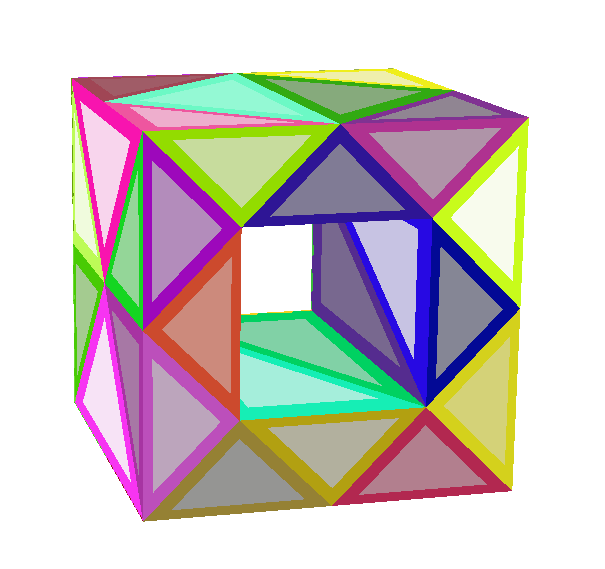
\includegraphics[width=.4\linewidth]{Testbed/poly2.png}
		\caption{Complexere figuur}
	\end{subfigure}
	\caption{Voorgedefinieerde polyhedra.}
	\label{fig: polyhedra}
\end{figure}
